\documentclass{beamer}
\usepackage[T1]{fontenc}
\usepackage[utf8]{inputenc}
\usepackage{lmodern}
\usepackage{listings}


\definecolor{ingorange}{rgb}{1.0,0.38,0.0}
\useoutertheme{tree}
\setbeamercolor{titlelike}{fg=ingorange}
\setbeamertemplate{itemize item}{\color{ingorange}$\blacktriangleright$}

\definecolor{dkgreen}{rgb}{0,0.6,0}
\definecolor{gray}{rgb}{0.5,0.5,0.5}
\definecolor{mauve}{rgb}{0.58,0,0.82}

\lstdefinestyle{Scala}{
  frame=tb,
  language=scala,
  aboveskip=3mm,
  belowskip=3mm,
  showstringspaces=false,
  columns=flexible,
  basicstyle={\scriptsize\ttfamily},
  numbers=none,
  numberstyle=\tiny\color{gray},
  keywordstyle=\color{blue},
  commentstyle=\color{dkgreen},
  stringstyle=\color{mauve},
  frame=single,
  breaklines=true,
  breakatwhitespace=true,
  tabsize=3,
}

\title{Categories in the wild}
\author{Wouter Stekelenburg}

\newcommand\hide[1]{}

\begin{document}
\lstset{style=Scala}
\begin{frame}
  \titlepage
\end{frame}

\hide{
\begin{frame}[plain]
\frametitle{Categories are like \dots}
Categories are like cats. It is easy to learn what they are, but that doesn't mean you understand them or can work with them without getting hurt.
\end{frame}
}

\section{Set up}
\begin{frame}[fragile]
\frametitle{Naked interface}

\begin{lstlisting}
trait Cassandra {
  def prepare(statement: String): PreparedStatement
  def prepare(statement: RegularStatement): PreparedStatement
  def execute(statement: String): Unit
  def execute(statement: Statement): Unit
}
\end{lstlisting}

\end{frame}

\begin{frame}[fragile]
\frametitle{Wrapped interface}

\begin{lstlisting}
trait Cassandra {
  def prepare(statement: String): F[PreparedStatement]
  def prepare(statement: RegularStatement): F[PreparedStatement]
  def execute(statement: String): F[Unit]
  def execute(statement: Statement): F[Unit]
}
\end{lstlisting}

\end{frame}

\section{Categorical specifications}

\begin{frame}[fragile]
\frametitle{Map}
\begin{lstlisting}
map: (X => Y) => F[X] => F[Y]

// map((x: X) => x)(y) === y
// map(f)(map(g)(y)) === map((x: X) => f(g(x)))(y)
\end{lstlisting}
\begin{center} 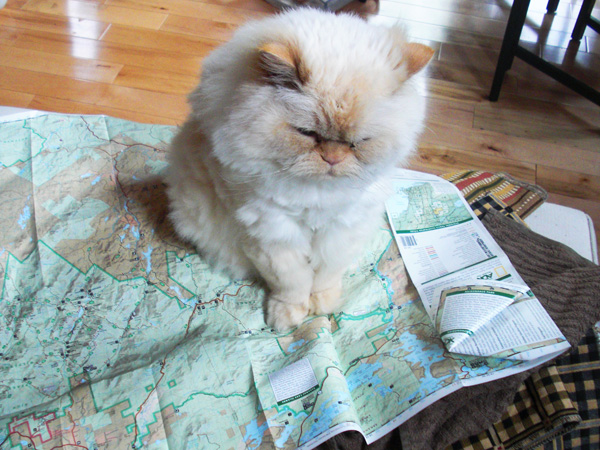
\includegraphics[height=3cm]{cat_map.jpg} \end{center}
\end{frame}

\begin{frame}
\frametitle{Functor}

\includegraphics{funktor.jpeg}
\end{frame}

\begin{frame}[fragile]
\frametitle{Zip}
\begin{lstlisting}
zip: (F[X],F[Y]) => F[(X,Y)]

// map(_._1)(zip(fx, fy)) === fx
// map(_._2)(zip(fx, fy)) === fy
// zip(map(_._1)(z),map(_._2)(z)) === z
\end{lstlisting}
\begin{center} 
\includegraphics[height=3cm]{cat_zip.jpg} \end{center}
\end{frame}

\begin{frame}[fragile]
\frametitle{Unit}
\begin{lstlisting}
unit: X => F[X]

// map(f)(unit(x)) === unit(f(x))
\end{lstlisting}
\begin{center} 
\includegraphics[height=3cm]{cat_unit.jpg} \end{center}
\end{frame}

\begin{frame}[fragile]
\frametitle{Applicative functor}
\begin{lstlisting}
map: (X => Y) => F[X] => F[Y]
zip: (F[X],F[Y]) => F[(X,Y)]
unit: X => F[X]
\end{lstlisting}
\begin{center} 
\includegraphics[height=3cm]{cat_applicative.jpg} \end{center}
\end{frame}

\begin{frame}[fragile]
\frametitle{Bind}
\begin{lstlisting}
bind: (X => F[Y]) => F[X] => F[Y]

// bind(f)(bind(g)(x)) === bind((y: X) => bind(f)(g(y))(x))
// bind(unit)(x) === x
// bind(f)(unit(x)) === f(x)

// map(f)(x) === bind((y: X) => unit(f(y)))(x)
// zip(x,y) === bind((x0: X) => map((y0: Y) => (x0, y0)))
\end{lstlisting}
\begin{center} 
\includegraphics[height=2cm]{cat_bind.jpg} \end{center}
\end{frame}

\begin{frame}[fragile]
\frametitle{Monad}
\begin{columns}
\begin{column}{0.6\textwidth}
\begin{lstlisting}
unit: X => F[X]
bind: (X => F[Y]) => F[X] => F[Y]
\end{lstlisting}
\end{column}
\begin{column}{0.4\textwidth}

\includegraphics[width=\textwidth]{cat_monad.jpg}
\end{column}
\end{columns}
\end{frame}


\section{Demo}

\begin{frame}
\frametitle{Demo}
\end{frame}

\section{Conclusion}

\begin{frame}
\frametitle{Summary}
`functor', `applicative functor' and `monad' specify interfaces that handle callbacks, in increasing power
\end{frame}

\end{document}
